\chapter{深度强化学习算法}
\section{引言}
本章将会对我们使用的机器学习算法原理进行论述包含强化学习中的\textit{Q}表学习和融入深度神经网络的DQN算法,并在前人基础上加入新的想法,将长短时记忆网络(LSTM)加入DQN中,并对网络结构进行相应优化,比如增加训练效率的duling方法和为了网络训练更稳定而加入的目标\textit{Q}网络。
\section{深度强化学习相关理论}
\subsection{\textit{Q}学习}
首先介绍强化学习,作为机器学习的一种,强化学习主要包括智能体(Agent),环境(Environment),状态(State),动作(Action),奖惩值(Reward)组成,如图\ref{fig:强化学习}所示。将其如认知无线电框架\ref{fig:认知无线电}相类比,可见结构较为相似,这也是我们认为可以使用强化学习方法解决频谱分配问题的原因之一。
\begin{figure}[htbp]
	\begin{minipage}{\textwidth}
		\centering
		\subfigure{\label{fig:强化学习}}\addtocounter{subfigure}{-2}
		\subfigure{\subfigure[强化学习框架]{\includegraphics[width=0.25\textheight]{强化学习}}}
		\hspace{1em}
		\subfigure{\label{fig:认知无线电}}\addtocounter{subfigure}{-2}
		\subfigure{\subfigure[认知无线电框架]{\includegraphics[width=0.3\textheight]{认知无线电框架}}}
		\hspace{1em}	
	\end{minipage}
	\vspace{0.2em}
	\caption{强化学习与认知无线电类比}\label{fig:强化学习类比认知无线电}
\end{figure}
整个过程是智能体与环境不断交互中进行的,在环境中,智能体执行一个动作后,与环境进行交互,环境依据选取的动作给出反馈(积极的或是消极的),智能体会依据反馈进行自我训练(例如\textit{Q}表更新或是神经网络权值改变等),随后,智能体会根据环境的反馈和新的状态按照一定的策略执行新的动作。如此循环往复,直至任务结束。强化学习目标是累积奖赏值的最大化,如式\ref{eq:强化学习目标}所示。强化学习的常见模型是标准的马尔可夫
\begin{equation}\label{eq:强化学习目标}
G_{t}=R_{t+1}+\lambda R_{t+2}+\cdots=\sum_{k=0}^{\infty}\lambda^{k}R_{t+k+1}
\end{equation}
决策过程,侧重于训练学习并在未遍历选择间的探索和已知最优化选择之间的平衡。与监督学习和非监督学习不同的是,强化学习不需要提前准备大量的训练数据,其训练数据是通过接收环境对动作的反馈而来,并由此进行模型更新。

\begin{figure}[h]
	\centering
	\includegraphics[width = 1.0\textwidth]{Q学习}
	\caption{\textit{Q}学习示意图}
	\label{fig:Q学习}
\end{figure}

强化学习中最为典型的就是\textit{Q}表学习算法,其算法结构如图\ref{fig:Q学习}所示。其中\textit{Q}-learning算法是\textit{Q}学习的核心算法。算法最终目标为找到一个使累积折扣奖赏最大的策略,如式\ref{eq:Q学习目标}所示。
\begin{equation}\label{eq:Q学习目标}
\underset{\pi}{\max }\mathbb{E}\left [ \sum_{t=0}^{H}\gamma^{t}R\left ( S_{t},A_{t},S_{t+1} \right )\mid\pi \right ]
\end{equation}
算法使用时间差分法(TD算法),同时融合蒙特卡洛(深度优先)和动态规划(广度优先)方法,能够进行离线学习。利用贝尔曼方程\ref{eq:贝尔曼方程}可以对符合马尔可夫决策过程的问题求解最优策略。每个状态的价值不仅取决于当前状态,还需要考虑后续状态的预估价值。
\begin{equation}\label{eq:贝尔曼方程}
\left\lbrace 
\begin{aligned}
V_{\pi(s)}=&\mathbb{E}\left ( U_{t}\mid S_{t=s} \right )\\
V_{\pi(s)}=&\mathbb{E}_{\pi}\left [ R_{t+1}+\gamma \left [ \cdots \right ]\mid S_{t=s} \right ]\\
V_{\pi(s)}=&\mathbb{E}_{\pi}\left [ R_{t+1}+\gamma V\left ( {s}' \right )\mid S_{t=s} \right ]
\end{aligned}
\right.
\end{equation}
绝大多数情况下我们使用价值函数$V_{\pi(s)}$表征某一策略下某个状态的价值,并使用动作价值函数$Q(s,a)$表征某一状态动作对对于整个问题的价值大小,也即在某一状态下采取某一动作的好坏,因此,\textit{Q}学习又被分类为基于价值的强化学习。最优状态动作函数如式\ref{eq:Q函数}所示。
\begin{equation}\label{eq:Q函数}
Q^{*}\left ( s,a \right )=\sum _{{s}'}P\left ( {s}'\mid s,a \right )\left ( R\left ( s,a,{s}' \right ) +\gamma\max _{{a}'}Q^{*}\left ( {s}' ,{a}'\right )\right )
\end{equation}
对公式直观的解释是当前的动作价值函数等于将执行完该动作之后所有可能达到的下一状态进行遍历,并借助贝尔曼方程将下一动作置换为对应奖赏和执行当前策略的最优动作时的动作价值函数的加和形式。以此引入当前策略下的下一状态的动作价值函数,形成迭代关系,通过训练使迭代趋于收敛。为了完成这样的迭代训练,我们需要引入\textit{Q}算法的学习机制,由公式\ref{eq:Q学习更新函数}给出。
\begin{equation}\label{eq:Q学习更新函数}
\left\lbrace 
\begin{aligned}
&Q_{k+1}\left ( s_{t},a_{t} \right )=Q_{k}\left ( s_{t},a_{t} \right )+\alpha_{k}E_{k}\\
&E_{k}=r_{t}+\gamma\max Q_{k}\left ( {s_{t}}' ,{a_{t}}'\right )-Q_{k}\left ( s_{t},a_{t}\right )
\end{aligned}
\right.
\end{equation}
当训练至损失函数$E_{k}$小于提前设定的一个较小的阈值$\epsilon$时认为迭代收敛,训练停止,此时\textit{Q}表成功建立,任意输入某一状态$s(t)$都可以由\textit{Q}表查询到对应的最优动作,也即完成了最优策略的寻找。
\subsection{深度\textit{Q}学习}
传统的\textit{Q}表学习对于拥有维度较小的状态空间和动作输出空间的问题有较好的解决效果,但其有一个瓶颈就是因为要使用一个表格储存所有的状态动作函数,当一个复杂问题拥有较高的输入状态维度和较大的动作输出维度时,\textit{Q}表学习就显得有些力不从心。一方面由于连续状态存在,表格索引这种离散化的描述方式使得智能体对于动作价值函数的描述变得精度不足。另一方面,大量的状态动作维度使得表格变得十分巨大,在训练时更新带来灾难性的计算复杂度和时间复杂度,在测试时对表格的遍历也变得十分困难。这些问题极大程度的限制了传统\textit{Q}学习在频谱分配相关问题上的应用。
\begin{figure}[h]
	\centering
	\includegraphics[width = 0.7\textwidth]{DQN}
	\caption{DQN算法示意图}
	\label{fig:DQN}
\end{figure}

近年来深度学习发展迅速,成为机器学习中最耀眼的成果,深度神经网络对于复杂状态的感知能力极为强大。有研究学者将深度神经网路的感知能力同强化学习的决策能力相结合,提出了深度强化学习\cite{mnih2013playing}概念,其中以DQN算法最为典型。DQN算法同传统\textit{Q}表学习算法最显著也是最核心的不同即为使用深度神经网络替代原有的\textit{Q}表格,使用深度神经网络对\textit{Q}函数进行近似,如图\ref{fig:DQN}所示。DQN以值网络作为评价模块,基于值网络的输出进行动作的选择。这里我们注意到DQN算法还加入了一个记忆单元,这个改变是由于深度神经网络训练的特殊性引起的。我们加入记忆单元储存每次交互产生的状态,动作,奖赏,下一状态组成的元组,并在训练时进行随机抽取,这样做的目的有两个,最主要的是打破输入数据间的相关性,降低网络陷入局部最优的概率,同时可以对数据进行自定义形式抽取,提高网络训练效率。这里对于误差函数的设置也较为特殊,类比监督学习,构建一个残差模型,我们将公式\ref{eq:Q学习更新函数}中的误差函数$E_{k}$作为训练优化目标,使用优化器利用梯度下降算法进行网络权值更新,随后进入下一步骤,多次与环境交互并训练,直至网络收敛,损失函数下降到设定阈值$\epsilon$之下,训练结束。

此外我们需要额外加入一个带有探索性质的动作选择策略,倘若在智能体通过环境交互过程中,智能体只选择当前网络给出的最优动作,有可能会使网络陷入局部最优的策略中,因为网络没有对未知动作进行探索,会导致记忆体内存储的历史经验不能完全包含相应问题的所有动作空间,这样的结果是我们所不愿见到的。为此,要利用$\epsilon-$贪心算法进行动作选择。算法核心是设置一个随训练轮次增加而逐步减小的阈值$\epsilon$,然后每次需要进行动作选取时生成一个随机数$p$,如果$p\leqslant \epsilon$此次动作选取使用随机探索方式选取,如果$p> \epsilon$选择网络输出的$\arg \max \left ( Q \right )$对应的最佳动作。

\section{长短期记忆网络}
科学家发现大脑皮层的解剖结构现实电流刺激信号可以在神经回路中循环存在,计算机科学家进行类比后提出反向回路设想。后来又有学者补充了循环神经网络的时间反向传播(BP Through Time, BPTT)算法,成为循环神经网络主要的学习方式。循环神经网络结构如图\ref{fig:循环神经网络}所示,其数学表达式如式\ref{eq:循环神经网络结构}所示。
\begin{figure}[h]
	\centering
	\includegraphics[width = 0.7\textwidth]{循环神经网络}
	\caption{循环神经网络结构}
	\label{fig:循环神经网络}
\end{figure}
\begin{equation}\label{eq:循环神经网络结构}
\left\lbrace 
\begin{aligned}
&O_{t}=g\left ( Vh_{t} \right )\\
&h_{t}=f\left ( Ux_{t} + Wh_{t-1} \right )
\end{aligned}
\right.
\end{equation}
其中$W$为网络各层连接的权值矩阵。$o_{t}$为相应时刻输出,$x_{t}$为相应时刻输入,$h_{t}$为神经节点状态值。网络采用基于时间的反向传播算法(BPTT)进行权值更新,这里数学推导颇为复杂,不作详谈。这种传统循环神经网络有一个缺点式由于长期依赖因素可能会导致梯度爆炸或消失,这时我们就需要其升级版本,长短期记忆网络(LSTM)。这里我们给出LSTM的网络结构示意图\ref{fig:LSTM示意图}。所有神经节点具有相同的结构,其核心是神经元状态,图中使用$C_{t}$表示,它贯穿整个神经元。
\begin{figure}[h]
	\centering
	\includegraphics[width = 1\textwidth]{LSTM}
	\caption{LSTM结构示意图}
	\label{fig:LSTM示意图}
\end{figure}
另外标注有$\sigma$矩形为神经元的遗忘门,是一个sigmoid函数同信息进行点乘,用来控制历史信息流入量。信息先经过第一个遗忘门,表示由神经元决定抛弃哪些信息如式\ref{eq:抛弃函数}所示。
\begin{equation}\label{eq:抛弃函数}
f_{t}=\sigma\left ( W_{f} \cdot \left [ h_{t-1},x_{t} \right ]+b_{f}\right )
\end{equation}
然后是一个输入门,决定为神经元状态新添加哪些信息,具体操如公式\ref{eq:LSTM输入公式}所示。使得当前神经元状态变为$C_{t}=f_{t}*C_{t-1}+i_{t}*\tilde{C}_{t}$。
\begin{equation}\label{eq:LSTM输入公式}
\left\lbrace 
\begin{aligned}
&i_{t}=\sigma \left ( W_{i} \cdot \left [ h_{t-1},x_{t} \right ] +b_{i}\right )\\
&\tilde{C}_{t}=tanh\left ( W_{C} \cdot \left [ h_{t-1},x_{t} \right ] +b_{C}\right )
\end{aligned}
\right.
\end{equation}
最后通过tanh函数进行激活,以此作为神经元的输出,如式\ref{eq:LSTM输出公式}所示。
\begin{equation}\label{eq:LSTM输出公式}
\left\lbrace 
\begin{aligned}
&o_{t}=\sigma \left ( W_{o} \cdot \left [ h_{t-1},x_{t} \right ] +b_{o}\right )\\
&h_{t}=o_{t}*tanh\left ( C_{t} \right )
\end{aligned}
\right.
\end{equation}
然后便是将LSTM加入传统深度神经网络之中,与DQN一同形成DRQN算法。这种深度强化学习因为加入了LSTM网络使得智能体可以通过历史信息对当前状态进行预测,可以更加有效的完成频谱智能分配任务。

\section{DRQN算法优化}
\subsection{Dueling DQN}
\begin{figure}[h]
	\centering
	\includegraphics[width = 1\textwidth]{dueling}
	\caption{加入Dueling方法的DRQN结构示意图}
	\label{fig:dueling结构图}
\end{figure}
在使用上文提出的深度强化学习解决频谱分配问题时,我们发现网络收敛速度不够快,智能体训练效率有限,通过参考文献\cite{8254101}提出的网络结构,发现需要改变输入网络结构。因为问题中包含某些比较差或比较好的状态,在这些状态下无论我们取什么动作都不会影响输出的奖赏。这时我们需要在现有网络基础上采取Dueling方法\cite{Wang2015Dueling}。该方法使用公式\ref{eq:dueling方法}表示。其中$V\left(\cdot\right)$表示只有状态决定的状态函数,$A\left(\cdot\right)$表示与动作状态相关的优势函数。更改后的整体网络结构如图\ref{fig:dueling结构图}所示。
\begin{equation}\label{eq:dueling方法}
Q\left ( a_{n}\left (t\right )\right )\leftarrow V + A\left ( a_{n}\left (t\right )\right )  
\end{equation}

\subsection{目标\textit{Q}网络}
加入dueling方法后的深度神经网络拥有了更高的训练效率和更新速度,但整个系统的稳定性却达不到我们的预期要求。为此,通过借鉴DeepMind在2015年提出的一种新型算法对网络框架进行了更新和调整。这里我们在原有DRQN网络上再加上一个结构和初始权值一模一样的深度神经网络,两者分别使用$Q_{value}$和$Q_{target}$表示。在训练时我们会固定住$Q_{target}$网络的权值参数,仅对$Q_{value}$网络进行网络的反向梯度传递和权值更新,然后在经历固定次数(取决于我们设定的超参数)训练后将$Q_{value}$网络中所有权值和偏置参数复制给$Q_{target}$网络,达到一个延迟更新的目的。下面我们通过具体数学推导解释这样操作的原因。在我们计算网络的损失函数(TD error)时,我们是通过计算$Q_{value}$和$Q_{target}$的输出插值得到的,如式\ref{eq:target weight}所示。
\begin{equation}\label{eq:target weight}
\Delta w=\alpha\left [ \left ( R+\gamma\max _{a} \hat{Q}\left ( {s}' ,a,w\right )\right )- \hat{Q}\left ( s ,a,w\right )\right ]\nabla_{w}\hat{Q}\left ( s,a,w \right )
\end{equation}
\begin{figure}[htbp]
	\begin{minipage}{\textwidth}
		\centering
		\subfigure{\label{fig:tensorboard_q_net}}\addtocounter{subfigure}{-2}
		\subfigure{\subfigure[$Q_{value}$网络结构]{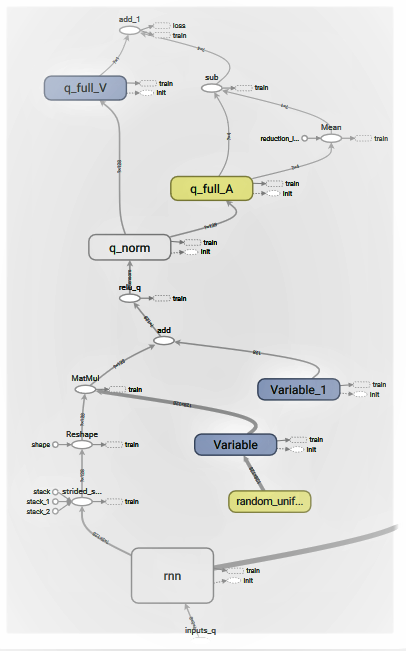
\includegraphics[width=0.25\textheight]{Q_net_tensorboard}}}
		\hspace{1em}
		\subfigure{\label{fig:tensorboard_q_target}}\addtocounter{subfigure}{-2}
		\subfigure{\subfigure[$Q_{target}$网络结构]{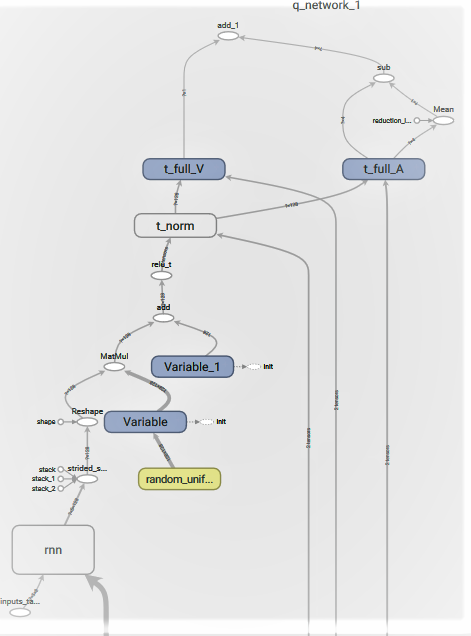
\includegraphics[width=0.3\textheight]{Q_target_net_tensorboard}}}
		\hspace{1em}	
	\end{minipage}
	\vspace{0.2em}
	\caption{Tensorboard中两网络结构图}\label{fig:target网络}
\end{figure}
在实际计算中,我们希望公式\ref{eq:Q学习更新函数}中$E_{k}$趋近于零,因此,令$Q_{value}$网络输出值为我们想逼近的\textit{Q}函数,$\gamma\max _{a} \hat{Q}\left ( {s}' ,a,w\right )$设为$Q_{value}$网络逼近的下一状态\textit{Q}函数,其加上奖赏$r(s,a)$形成训练标签。问题在于该标签中$\gamma\max_{a}\hat{Q}\left ( {s}' ,a,w \right )$部分同网络权值具有极大的相关性,也就是每次训练标签同训练目标向同一方向改变,会产震荡现象,影响训练收敛及其稳定性。因此我们需要额外引入一个固定的标签,也即$Q_{target}$网络形成的标签,使用独立的参数来预测TD-error,并在固定次数步骤后对权值进行复制来进行训练,如公式\ref{eq:new target}所示。
\begin{equation}\label{eq:new target}
\Delta w=\alpha\left [ \left ( R+\gamma\max _{a} \hat{Q}\left ( {s}' ,a,w^{-}\right )\right )- 	\hat{Q}\left ( s ,a,w\right )\right ]\nabla_{w}\hat{Q}\left ( s,a,w \right )
\end{equation}
在代码层面实际操作时,我们需要构建两个相同结构网络,但分别放置于不同的命名空间下,以此做到权值的独立性,这里我们对其Tensorboard结构图\ref{fig:target网络}进行展示。

\section{本章小结}
在这一章中,我们对深度强化学中\textit{Q}学习,DQN以及LSTM进行了简要介绍,通过类比认知无线电同强化学习相似之处,给出使用机器学习解决频谱分配问题的方案,并依据LSTM的历史信息感知判断和DQN对于MDP问题的高效决策能力,引出解决频谱分配问题需要使用的DRQN结构,并在此基础上加入Dueling方法提高算法训练效率,使用固定的$Q_{target}$网络保证网络的稳定性。对论文所使用的算法进行概要介绍以及必要的数学推导,便于从原理上理解机器学习解决相关问题的底层机理,为后文结果分析提供必要的理论支撑。

\chapter{基于空天地一体化的频谱资源分配问题背景及建模}
\section{引言}
空天地一体化通信框架融合卫星通信,空基无人机(UAV),地面移动通信为一体,三者优劣互补,可为未来通信提供更广覆盖,更低延时,更大带宽,更高可靠的新一代通信服务。对于传统地面蜂窝网结构进行改进,提出基于分簇模型的新型框架,使用户在作为服务中心的同时成为资源分配中心,可以更自主,更便捷,也更高效合理的实现资源分配。本章将对空天地一体化模型进行展示,并着重介绍我们提出的分簇模型框架,并将对设计的相关问题的数学模型进行叙述。

\section{空天地一体化新型通信框架模型的建立}
对于现有传统通信系统如图\ref{fig:现有框架}所示。主要包括卫星通信系统,空基无人平台以及地面通信网络。其中地面段通信系统较为完善,而对于包含高空平流层的空天地一体化的通信系统模型研究还并不完善,这里我们需要对于异构系统进行简化。
\begin{figure}[h]
	\centering
	\includegraphics[width = 0.8\textwidth]{一体化框架}
	\caption{现实情况下异构系统通信框图}
	\label{fig:现有框架}
\end{figure}

简化后的模型如图\ref{fig:简化模型}所示。卫星可以直接与地面终端进行通信,同时也可以经由空中无人平台进行中转和广播,由于设计协议复杂,我们现就问题主要矛盾,即地面段异构系统的频谱分配进行研究,在算法较为成熟时再考虑空间段的具体细节。

\begin{figure}[h]
	\centering
	\includegraphics[width = 0.7\textwidth]{简化模型}
	\caption{简化后的新型通信框架}
	\label{fig:简化模型}
\end{figure}

\section{分簇模型}
\subsection{分簇模型结构}
这里不同与传统的蜂窝网概念,我们创新性的提出用户为中心自组织式的分簇模型。在我们构建的新型通信模型下,作为中介节点的不止有基站,可能还有一些设备能力较强的终端用户形成自组织式的小小区,我们将之称为簇头,现在主要讨论簇内与簇间在考虑同频干扰情况下的频谱分配算法的优化。模型构建类似于地面移动通信的蜂窝网模型,但与之不同点在于基站的角色由簇头承担,簇头可以是现存基站,也可以是具有较强计算能力的移动终端,分簇模型如图\ref{fig:分簇模型结构图}所示。这里我们假设每个簇头可能连接多个簇内用户为他们提供信息传输服务,每个用户也可能同时连接多个簇头,通过训练后的分布式智能体( 簇内用户)可以自主选择连接哪些簇头,然后在被告知共用用户数量后再自主选择特定信道申请分配。这些都结束后,中心智能体(簇头)会根据申请连接情况进行智能功率控制,以此达到网络总传输速率最高。
\begin{figure}[h]
	\centering
	\includegraphics[width = 0.9\textwidth]{分簇模型结构图}
	\caption{分簇模型结构示意图}
	\label{fig:分簇模型结构图}
\end{figure}

\subsection{分簇模型建立原因及意义}
关于分簇原因我们这里列出如下:

(1) 动态的网络:用户和基站都将具有相当的移动性。用户的移动性不再赘述,基站的移动性主要是指一体化组网构架下,为了弥补地面网络带宽受限的问题而引入了平流层的飞艇作为移动的基站。在这种状况下,不得不通过分簇来解决动态性的问题。

(2) 分布式的系统:未来系统可能是分布式的,之前的工作也已经说明,分布式系统中的用户联系松散,需要根据特定的情况来保持和特定用户群体的联系。因此,分簇和分布式的系统也是密切相关的。

(3) 用户需求多样化的网络:用户对通信的需求大相径庭,需要打破小区不重叠、 在哪个小区用哪个基站的限制,让用户自由选择节点、甚至组成以自己为中心的簇,自主地调配资源,为自己服务。

\section{问题的数学模型}
这里我们对相关问题进行简化和抽象,并进行数学建模,为后续问题解决提供体系化的理论支持。首先我们给出整个问题的完整流程图如\ref{fig:整体流程图}所示。
\begin{figure}[htbp]
	\centering
	\includegraphics[width = 0.9\textwidth]{分簇频谱分配算法}
	\caption{异构系统频谱智能分配整体流程图}
	\label{fig:整体流程图}
\end{figure}

待解决问题主要分为三个部分,实现簇头自主选择部分,我们简化问题为基于历史信息的相关信道状态预测问题,定义为部分观测的马尔可夫决策过程(POMDP)。然后是实现分布式多用户冲突避免问题,我们建模为纳什均衡问题,也称非合作博弈均衡,在仅知道竞争用户数量情况下通过训练使智能体达到纳什均衡状态。最后是功率控制部分,我们建模为认知无线电下次级用户的功率退避问题。

对于簇头的选择是用户依据历史信息对不同簇头当前转发状态与能力的估计,在之前的时隙中(timeslot),用户在每个时间隙发出信息传输请求,得到信息传输结果观测值(ACK),以此估计当前簇头转发状态好坏,输出一个布尔值(0/1),这里假设不同簇头之间是相关的,由于不能完全知晓当前簇头状态转移模式,因此是一个部分观测马尔可夫决策过程,如表格\ref{tab:马尔可夫分类}所示。对于挑选簇头问题可以建模为一个$2^{N}$状态的马尔科夫链,\textit{N}表示用户可连接簇头数目,状态空间为$S=\left\{S_{1},\cdots,S_{2^{N}}\right\}$,其中每个$S_{i}$,为一个长度为\textit{N}的向量,表示每个簇头当前状态。用户通过历史信息进行预测,并更新自身的系统状态分布推测$\Omega \left ( t \right )=\left [ \omega _{S_{1}} \left ( t \right ),\cdots,\omega _{S_{2^{N}}} \left ( t \right )\right ]$,每个向量元素表示系统位于当前状态概率,并依据此估计给出最优动作选择向量$a(t)$并获取ACK,以此根据公式\ref{eq:簇头选择更新公式}(式中$\mathbb{I}\left(\cdot\right)$为指示函数)更新系统状态猜测向量\cite{8303773}。
\begin{equation}\label{eq:簇头选择更新公式}
\hat{\omega }_{S_{i}}\left ( t \right )=\left\{
\begin{aligned}
\frac{\omega _{s_{i}\left ( t \right )}\mathbb{I}\left ( S_{ik}\left ( t \right ) =1\right )}{\sum_{i=1}^{2^{N}}\omega _{s_{i}\left ( t \right )}\mathbb{I}\left ( S_{ik}\left ( t \right ) =1\right )}& & a(t)=k,o(t)=1\\
\frac{\omega _{s_{i}\left ( t \right )}\mathbb{I}\left ( S_{ik}\left ( t \right ) =1\right )}{\sum_{i=0}^{2^{N}}\omega _{s_{i}\left ( t \right )}\mathbb{I}\left ( S_{ik}\left ( t \right ) =0\right )}& & a(t)=k,o(t)=0
\end{aligned}
\right.
\end{equation}
然后将猜测向量与每个簇头不同概率分布组成的状态转移矩阵\textit{P}做乘积得到下一状态概率矩阵$\Omega \left ( t+1 \right )$,以此达到长期累积折扣奖赏最大的优化目标,获得最优策略,如公式\ref{eq:簇头选择长期奖励}所示。其中$R_{\pi\left ( \Omega \left ( t \right ) \right )}\left ( t \right )$为t时刻在当前状态$\Omega \left ( t \right ) $下,最佳策略$\pi^{*}$采取动作后得到的奖赏。折扣因子$\gamma$为介于0和1之间的数,用来表示长期奖励对总任务的重要程度。
\begin{equation}\label{eq:簇头选择长期奖励}
\pi ^{*}= \underset{\pi }{\arg \max}\mathbb{E}_{\pi}\left [ \sum_{t=1}^{\infty }\gamma ^{t-1} R_{\pi\left ( \Omega \left ( t \right ) \right )}\left ( t \right )\mid \Omega \left ( 1 \right )\right ]
\end{equation}
当簇头间相互独立且簇头状态转移概率分布形式一致时,每个用户基于自身的贪心算法即为最优策略\cite{Ahmad2009Optimality},但对于簇头间相互关联且变化概率分布未知的情况下这种算法得到的结果并不是最优化的,且由于簇头间相关性,该问题为一个PSPACE-hard问题\cite{8303773},很难通过传统算法得到精确解。
\begin{table}[htbp]
	\caption{马尔可夫模型类别}\label{tab:马尔可夫分类}
	\vspace{0.5em}\centering\wuhao
	\begin{tabular}{cccc}
		\toprule[1.5pt]
		名称 & 状态可见性 & 是否考虑动作 & 英文缩写 \\
		\midrule[1pt]
		马尔科夫链 & 状态完全可见 & 不考虑动作影响 & MC \\
		马尔可夫决策过程 & 状态完全可见 & 考虑动作影响 & MDP\\
		隐马尔可夫模型 & 状态不完全可见 & 不考虑动作影响 & HMM \\
		部分观测马尔可夫决策过程 & 状态不完全可见 & 考虑动作影响 & POMDP \\
		\bottomrule[1.5pt]
	\end{tabular}
\end{table}


对于分布式多用户对有限信道的竞争问题建模为纳什均衡问题。这里给出纳什均衡的定义在博弈$ G=\left \{ S_{1},\cdots,S_{n}:U_{1},\cdots,U_{n}\right \}  $中,每个博弈方采取一个策略,组成一个策略集合$\left\{S_{1}^{*},\cdots,S_{n}^{*}\right\}$,对于其中任意一个博弈成员$i$的策略$S_{i}^{*}$都是对其余博弈者采取策略组合$\left\{S_{1}^{*},\cdots,S_{i-1}^{*},S_{i+1}^{*},\cdots,S_{n}^{*}\right\}$的最佳应对策略,也即$U_{i}\left \{ S_{1}^{*}, \cdots ,S_{i}^{*},\cdots,S_{n}^{*} \right \}\geqslant U_{i}\left \{ S_{1}^{*},\cdots ,S_{ij}^{*},\cdots,S_{n}^{*} \right \}$对于任意$S_{ij}\in S_{i}$恒成立,我们称对应的策略集合为$G$的一个纳什均衡。通俗来讲就是其他竞争对手不改变自身竞争策略时候,自己不改变当前策略才会获取利益最大值,也就是达到平衡状态。对于信道竞争问题来说,即为在分布式用户间不进行合作式信息交流前提下达到平衡状态的问题。这里我们使用$\mathcal{N}=\left \{ 1,2,\cdots,N \right \}$表示簇内竞争用户然后使用集合$\mathcal{K}=\left \{0,1,2,\cdots,K \right \}$表示选择的信道(如果选择动作为0则表示用户在此时隙选择避让,不进行信息传递),在每个时隙,同一簇内不同用户选择一个簇头可提供信道发出信息传输请求,如果和其他用户不发生冲突则返回成功传输信号(ACK),反之亦然。目标仍然是达到长期总传输成功率最高。这里我们仍然使用带有折扣系数$\gamma$的累积奖赏作为优化目标,如式\ref{eq:冲突避免奖赏公式}所示。
\begin{equation}\label{eq:冲突避免奖赏公式}
R_{n}=\sum_{i=1}^{N}\sum_{t=1}^{\infty }\gamma ^{t-1}r_{n}\left ( t \right )
\end{equation}
由于用户间不能相互通信,所以普通算法对于这种问题只能使用随机信道选取方式,导致信道出现空闲或冲突,致使频谱利用效率降低,本文将使用深度强化学习解决这一问题。

对于多用户功率功率控制问题,我们将其设定为在认知无线电框架下的次级用户的功率退避问题。在完成簇头选择和信道选择后,簇头和簇内用户成功建立通信链路,但由于多用户的存在以及用户移动变化等因素,如果不采取相应的动态功率控制肯能导致同频干扰或是邻频干扰对信息传递造成巨大干扰,降低通信服务质量。简化起见,我们考虑簇内有个用户,并将其中一个假设为主用户(PU, primary user),另一个为次级用户(SU, secondary user),且每个用户都拥有自己的发射机($T_{X_{1}},T_{X_{2}}$)与接收机($R_{X_{1}},R_{X_{2}}$),两者属于非合作型共存方式,主用户不需要考虑次级用户,并且仅依据自己固定的原有功率策略进行功率调整。次级用户不知道主用户通讯功率及其功率策略,需要通过感知周围环境对主用户功率变化产生响应,及时调整自己的功率参数,以达到共同通信目的。这里需要特别提出的是,虽然主用户与次级用户不产生直接信息交流,但次级用户功率调整会通过环境变化引起主用户做出功率改变,也即客观上两者会产生相互作用。方便起见,我们假设两者同步进行功率调整,拥有相同时间基线。同时有感应节点部署在环境中获取接收信号强度(RSS, received signal stength),协助次级用户估计主用户传输状态。我们使用信干噪比SINR表示各用户QoS,如公式\ref{eq:SINR}所示,式中$h_{ij}$表示对应信道增益,$N_{i}$为对应噪声功率,主用户功率策略\cite{Grandhi1998Constrained}为如下公式所示\ref{eq:传统功率策略}。式中$D\left ( \cdot  \right )$为离散式功率选择函数,选取离散功率集合以$\mathcal{P}_{1}\triangleq\left \{ p_{1}^{p},\cdots,p_{L_{1}}^{p} \right \}$表示。$SINR_{1}(k)$为主用户测量得到的信干噪比,$p_{1}(k)$为主用户选择的功率。环境状态使用$p_{n}^{r}(k)=p_{1}(k)g_{1n}+p_{2}(K)g_{2n}+w_{n}(k)$进行描述,$p_{1}(k)g_{1n},\;p_{2}(K)g_{2n}$分别表示两用户发射功率同各自增益乘积,$w_{n}(k)$表示零均值高斯白噪声。
\begin{equation}\label{eq:SINR}
SINR_{i}=\frac{\left \| h_{ii} \right \|^{2}p_{i}}{\sum_{j\neq i}\left \| h_{ji} \right \|^2p_{j}+N_{i}}\; i=1,2 
\end{equation}
\begin{equation}\label{eq:传统功率策略}
p_{1}\left ( k+1 \right )=D\left ( \frac{\eta _{1}p_{1}\left ( k \right )}{SINR_{1}\left ( k \right )} \right )
\end{equation}
随后次级用户在智能体决策下选择一个功率集合$\mathcal{P}_{2}\triangleq\left \{ p_{1}^{s},\cdots,p_{L_{2}}^{s} \right \}$中的功率进行信息传输。当两用户都满足QoS要求($SINR_{i}\geqslant\eta_{i}$)时,此时刻返回奖赏为1,最终目标为整体长时累积奖惩最大化。
\section{本章小结}
在这一章节中,我们对整个问题的背景框架以及整体算法流程进行了介绍,并提出一种基于分簇理论的新型通信框架,在此基础上对于问题涉及的簇头选择,信道分配,功率控制这三方面进行了具体的数学语言描述,分别建模为部分观测马尔可夫决策过程,纳什均衡问题以及认知无线电框架下次级用户的功率退避问题,形成一个完备严密的逻辑体系,为后续工作奠定理论基础。









\chapter{异构系统频谱智能分配}
\section{引言}
在介绍了使用的机器学习算法及问题背景和数学模型之后,本章将对于基于分簇模型的异构系统频谱智能分配问题分为簇头选择,信道选择,功率控制三方面进行具体阐述以及使用Python配合Tensorflow平台进行算法仿真验证的结果展示以及分析,最后对本文使用的算法进行性能评估,提出存在不足并指出后续工作方向。

\section{DRQN算法流程及代码实现}
在结合LSTM以及DQN算法上形成的DRQN网络上进行Dueling和加入$Q_{target}$网络操作后我们给出一个完整DRQN的算法,如算法\ref{alg:DRQN}所示。
\begin{algorithm}[htb]  
	\caption{带有目标网络及经验回放策略的DRQN算法 }  
	\label{alg:DRQN}  
	 \begin{algorithmic}[1]  
		\Require  
		可交互环境类$ENV$;DRQN智能体$Agent$;储存体$Memory$;  
		\Ensure  
		智能体选取的输出动作集合$action$;  
		\State 初始化储存体$Memory$; 初始化智能体$Agent$中$Q_{value}$和$Q_{target}$网络的权值参数$w$和$w^{-}$;
		初始化环境状态,以随机动作方式生成输入状态$s_{t}$; 
		\State 将状态输入DRQN网络中,获取动作价值向量$Q$;  
		\State 使用前文介绍的$\epsilon -$贪心算法选取动作$a_{t}$; 
		\State 将该动作输入环境交互器$ENV$,获取动作对应奖励$r$,并生成下一状态$s_{t+1}$;
		\State 令$s_{t}=s_{t+1}$;将$s_{t},a_{t},r_{t},s_{t+1}$存入储存体中; 
		\State 当储存体中数据长度达到训练要求时开始网络训练过程; 从储存体中随机抽取固定数量的历史数据;  
		\State 将$s_{t}$输入$Q_{value}$网络,得到$Q$值;将$s_{t+1}$输入$Q_{target}$网络,加上$r_{t}$得到$target$值;
		\State 利用公式\ref{eq:new target},$\Delta w=\alpha\left [ \left ( R+\gamma\max _{a} \hat{Q}\left ( {s}' ,a,w^{-}\right )\right )- 	\hat{Q}\left ( s ,a,w\right )\right ]\nabla_{w}\hat{Q}\left ( s,a,w \right )$计算权值的反向传播梯度;
		\State 使用ADMA优化器进行$Q_{value}$网络的$w$更新;
		\State 每隔固定训练次数$n$就将$Q_{value}$网络的$w$传递给$Q_{target}$网络的权值参数$w^{-}$;
		\State 重复上述2至10操作至任务结束; \\
		\Return $Action$,$r$的累积奖赏$reward$;  
	\end{algorithmic}  
\end{algorithm}  
在使用Python3.6具体实现相应代码时,我将智能体设置成‘类’形式(Class),将函数和参数初始化包含在类中,借助Tensorflow编写神经网络搭建部分,利用张量间的矩阵乘法与加法实现全连接神经网络的构建。对于记忆体部分采用字典形式进行智能体与环境交互过程信息的储存,采取堆栈弹出和随机读取方式实现之前提到的经验回放策略。至于反向训练部分,使用Tensorflow自带的Adma优化方式进行梯度的反向传播,并进行节点权值的更新,在网络收敛后结束训练循环。随后将结果使用Pandas工具转换为.csv为后缀的数据文件储存,通过matplot.pyplt函数库绘制性能曲线,并进行分析。

\section{簇头选择}
\subsection{基于DRQN的簇头选择}
根据前文叙述的内容,用户在分簇模型下首先要在备选连接簇头集合$\mathcal{H} \triangleq \left \{ h_{1} ,h_{2},\cdots,h_{n}\right \}$中,依据自身信号传输要求选取最适合自身的相应簇头$h_{i}^{*}$,与之建立通信链路,进行信息传递。算法性能选用一定时间后用户自身传输信息成功比例表示,同时我们使用随机选择方式在备选簇头中任意选取簇头进行通信链路建立,统计同等情况下算法成功率。这里比较特殊的一点是不同簇头的状态变化间是相关的,这个设定主要考虑分簇模型中一些移动用户也会成为潜在簇头,由此不同于传统地面基站作为中介节点的蜂窝网构架下不同基站间相互影响由于距离较大的因素较小,所以可以忽略基站间影响。但对于我们的分簇模型,不同小簇头间距离较近,且可能进行业务协同,由此必须假定不同簇头间是紧密相关的,对于这种相关的多簇头未知变化规律的预测问题需要让智能体通过历史信息获得预测当前状态的能力,同时有需要让智能体拥有长期奖赏最大化的决策能力,无疑前文介绍的DRQN方法是最合适的解决工具。

具体实现多簇头联合相关状态变化这一目的,我们借鉴文章\cite{8303773}的思路,进行簇头状态相关性变化构造。进行仿真时,我们假设有16个备选簇头,将这些簇头随机划分到几个子集中,并将转移概率固定为$P=0.9$,最初状态下随机假定一个集合为活跃簇头集合,该集合内所有簇头均为可用的,活跃的,用户选取相应簇头进行信息传输时可以得到成功反馈($ACK=1$),在每个时隙开始前,活跃集合序号会依据固定的转移概率按照事先规定好的随机顺序转移至下一序号对应的簇头集合,激活其中所有簇头,以此实现簇头的相关动态状态转变,如算法\ref{alg:headstate}所示。
\begin{algorithm}[htb]  
	\caption{簇头相关动态状态转移算法}  
	\label{alg:headstate}  
	\begin{algorithmic}[1]  
		\Require  
		 可用簇头集合$\mathcal{H}$;状态转移概率$P$; 划分集合数$K$; 
		\Ensure  
		 备选簇头状态向量$S$;  
		\State 初始化随机簇头分配集合$\mathcal{T}\triangleq\left \{ t_{1}\triangleq\left \{h_{a},\cdots,h_{b}\right \} ,\cdots,t_{K}\triangleq\left \{h_{c},\cdots,h_{d}\right \}\right \}$;
		\State 随机选取一个集合为初始簇头激活集合,如$t_{i}$;				
		\State 在每个时隙开始时,生成一个随机数$\epsilon$,如果$\epsilon>P$,将当前激活集合取消激活,激活下一集合$t_{j}$;反之保持当前状态;  
		\State 将该时隙全部簇头状态存入簇头状态向量中;
		\State 重复上述3,4操作,至任务结束; \\
		\Return 簇头状态向量$S$;  
	\end{algorithmic}  
\end{algorithm}  
按照这种算法我们生成簇头状态图,如图\ref{fig:簇头状态}所示。图中选取前15个时隙作示意。图中可以明显看到簇头间变化的相关性,比如簇头10和簇头11变化规律一致,6和7变化规律一致。且可以看出簇头变化是较为剧烈的,这对于不知道簇头变化规律的申请用户来说想实现连续成功接入是较为困难的,但通过使用DRQN网络则可以较为出色的完成这一任务。
\begin{figure}[htbp]
	\centering
	\includegraphics[width = 0.9\textwidth]{簇头状态}
	\caption{相关簇头状态变化示意图}
	\label{fig:簇头状态}
\end{figure}


\subsection{簇头选择结果展示及分析}
在完成簇头变化状态建立之后需要对DRQN网络输入和输出进行调整,并使其可以同我们编写的环境模型进行交互。我们设置仿真超参数如表\ref{tab:超参数}所示。
\begin{table}[htbp]
	\caption{DRQN网络超参数设置}\label{tab:超参数}
	\vspace{0.5em}\centering\wuhao
	\begin{tabular}{cc}
		\toprule[1.5pt]
		超参数名称 & 仿真设置值 \\
		\midrule[1pt]
		探索概率$\epsilon$ & 0.1 \\
		训练单批次数据量 & 64\\
		LSTM时间步长 & 5 \\
		全连接层数 & 3 \\
		全连接层节点数 & 200 \\
		全连接层激活函数 & ReLU \\
		学习率 & $10^{-5}$ \\
		折扣因子$\gamma$ & 0.85 \\
		\bottomrule[1.5pt]
	\end{tabular}
\end{table}
我们将此前$K$步采取的动作和得到的传输反馈合并为一个向量做为状态输入DRQN中,动作输出设置为当前状态下预测信道序号,奖赏对应于采取该信道进行通信时成功与否的(ACK)反馈信息。然后使用算法\ref{alg:DRQN}开始仿真。同时给出随机选择方式结果用以对比算法性能。首先利用Tensorboard工具给出训练过程中的损失函数图\ref{fig:簇头训练loss}。 
\begin{figure}[htbp]
	\centering
	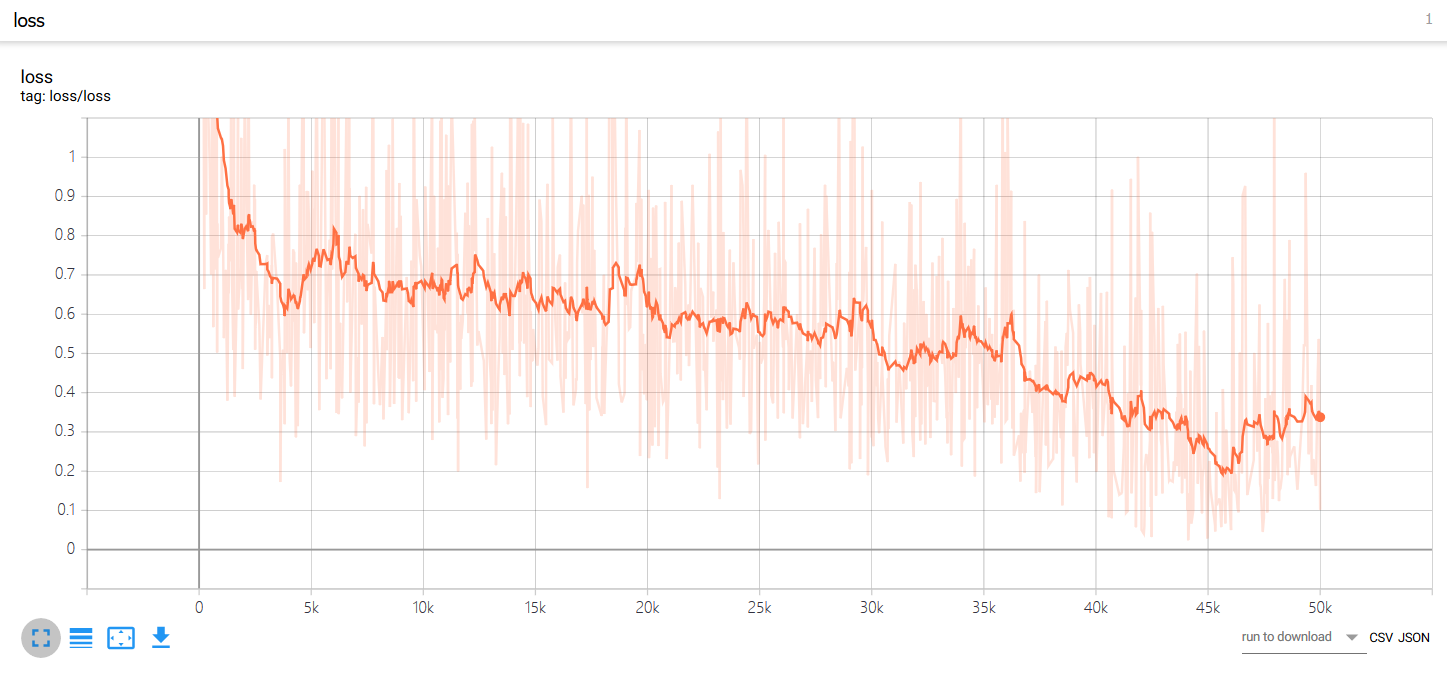
\includegraphics[width = 1\textwidth]{频道选择,损失,tensorboard}
	\caption{Tensorboard训练损失曲线图}
	\label{fig:簇头训练loss}
\end{figure}
由训练损失曲线可以看出随着训练次数的增加,训练损失逐渐降低,表明我们的训练是较为有效的,此外,在训练结束后对网络模型进行验证时损失曲线稍有上升,我的理解是训练有轻微过拟合问题导致的负增益,但这仍是可接受的,下面对输出结果进行展示,并对算法性能进行分析。

首先我们给出两种算法给出的簇头选择,如图\ref{fig:簇头动作对比}所示。对于DRQN智能体给出的结果具有十分明显的簇头倾向性,表明智能体通过对于历史信息的学习对于簇头状态拥有自己的判断,相比于随机算法的选择显然是更为合理的。

\begin{figure}[htbp]
	\begin{minipage}{\textwidth}
		\centering
		\subfigure{\label{fig:簇头动作DRQN}}\addtocounter{subfigure}{-2}
		\subfigure{\subfigure[DRQN算法的簇头选择展示]{\includegraphics[width=0.5\textheight]{簇头动作DRQN}}}
		\hspace{1em}
		\subfigure{\label{fig:簇头动作random}}\addtocounter{subfigure}{-2}
		\subfigure{\subfigure[random算法的簇头选择展示]{\includegraphics[width=0.5\textheight]{簇头动作random}}}
		\hspace{1em}	
	\end{minipage}
	\vspace{0.2em}
	\caption{随机算法同DRQN算法选取簇头对比}\label{fig:簇头动作对比}
\end{figure}

\begin{figure}[htbp]
	\centering
	\includegraphics[width = 0.7\textwidth]{簇头条形图}
	\caption{DRQN及随机算法簇头选择概率情况}
	\label{fig:簇头条形图}
\end{figure}
这里我们给出不同簇头在两种算法下的选取统计概率,对于个别簇头高概率选取的策略是否有效需要通过两种算法不同的信息传输成功情况来体现。因此我们给出两种算法对于同一情况给出的不同选择的传输反馈(ACK)来表示,图\ref{fig:簇头对比折线}展示随时间进行,使用DRQN算法的智能体累积奖赏值高于随机选取算法。具体传输结果如图\ref{fig:簇头奖励对比}所示。图中绿色方格代表用户在该时刻成功选择了合适的簇头,成功进行簇头用户间链接,可从肉眼直观看出使用DRQN算法的簇头选择策略成功率显著高于使用随机选取方式的智能体。这也证明了我们的算法是有效果的,进行了正向优化。
\begin{figure}[htbp]
	\centering
	\includegraphics[width = 0.7\textwidth]{簇头对比折线}
	\caption{DRQN同随机算法簇头选择成功率对比曲线}
	\label{fig:簇头对比折线}
\end{figure}

\begin{figure}[htbp]
	\begin{minipage}{\textwidth}
		\centering
		\subfigure{\label{fig:簇头奖励DRQN}}\addtocounter{subfigure}{-2}
		\subfigure{\subfigure[DRQN算法的簇头选择展示]{\includegraphics[width=0.5\textheight]{簇头奖励DRQN}}}
		\hspace{1em}
		\subfigure{\label{fig:簇头奖励random}}\addtocounter{subfigure}{-2}
		\subfigure{\subfigure[random算法的簇头选择展示]{\includegraphics[width=0.5\textheight]{簇头奖励random}}}
		\hspace{1em}	
	\end{minipage}
	\vspace{0.2em}
	\caption{随机算法同DRQN算法选取簇头成功情况对比}\label{fig:簇头奖励对比}
\end{figure}


\section{信道选择}
\subsection{基于DRQN的分布式用户信道选择}
在每个用户都选取自己理想连接簇头后,就需要执行信道分配动作。因为一个小簇头可提供信道数量并不太多,在用户饱和场景下难免会产生信道申请冲突,用户竞争信道会导致双方信息传输失败,致使信道利用效率大大降低,因此用户间的冲突避免就显得尤为重要。由于是异构网络下的频谱共享,不同用户可能分属于不同的网络系统,因此这里我们需要假设用户间不进行信息交流,在这种情况下如果使用中央分配方式可以轻松解决该问题,但我们构建的分簇模型中簇头除了地面固定基站外还可以是空中无人机平台(UAV)以及地面段部分用户,这时如果将信道分配工作全部交由中心节点进行处理和组织,会给簇头带来较大的计算任务负担,影响其信息传输业务。其次,由于我们考虑的是多用户动态频谱分配,用户具有移动性,进行中央式频道管控面临频繁的分配策略变更问题,任意用户进出都将要求中心节点进行重新规划和分配,在簇头和用户高密度的未来通信场景下显然是不利的。这里我们需要采取分布式智能方式,自主选择申请信道,并配合自身的簇头选择完成完全以用户自身为中心的自主化资源申请与分配。这样可以充分体现分布式策略优势,同时也最大化分簇模型的用户QoS体验,实现每个用户都成为"中心"的资源分配思想。
\begin{figure}[htbp]
	\centering
	\includegraphics[width = 0.7\textwidth]{信道动作随机}
	\caption{随机算法下用户选择信道结果}
	\label{fig:信道随机动作}
\end{figure}

分布式智能决策设定让用户在对其他用户选择频道未知状态下如何做出最优信道选择被建模为一个经典的纳什均衡问题。在这种信息不对称情况下进行动作选择颇为困难,首先我们给出随机选取方式下的信道分配结果。进行仿真时为简便起见我们设置三个竞争用户,共同分配两个可用信道($channel_{1},channel_{2}$),每个用户在每个时隙选择一个自己的申请信道动作,这里我们用($0,1,2$)来表示,其中$0$表示用户在当前时隙状态下不进行信息传递,选择避让,$1$和$2$则表示选取对应信道进行信息传输,结果如图\ref{fig:信道随机动作}所示。对冲突信道申请检测并判定为信息传输失败,对成功的信道选择进行绘制,结果如图\ref{fig:信道成功随机}所示。
\begin{figure}[htbp]
	\centering
	\includegraphics[width = 0.7\textwidth]{信道成功随机}
	\caption{随机算法下用户选择信道成功结果}
	\label{fig:信道成功随机}
\end{figure}
显然,用户任意选择会导致大量冲突产生,降低频谱效率,这时我们就需要DRQN算法进行智能体训练及优化。在应用DRQN算法解决该问题时,我们仍然将多步历史决策动作和观测信息结果作为网络的输入,将选取的申请信道作为动作,将该动作是否与其他用户发生冲突作为反馈信息,也即奖励。进行具体仿真时使用DRQN算法,如算法\ref{alg:DRQN}所示。但是这里在具体仿真时出现了一些问题,比如使用整体网络累计奖赏作为每个用户评价指标时,我们成为用户合作模式,在该模式下会出现某一用户始终选择回避,不进行信息传递,这显然是不公平的,为此我们对单个用户训练时奖赏值进行修改,使其训练时使用竞争模式,这样在最终整体网络总传输效率不变的情况下,可以最大程度满足用户间的公平性。
\begin{algorithm}[htb]  
	\caption{用户竞争奖赏算法}  
	\label{alg:headstate}  
	\begin{algorithmic}[1]  
		\Require  
		可用信道集合$\mathcal{H}$; 
		\Ensure  
		信道选取动作向量$S$;  
		\State 依据DRQN算法选取某一信道作为申请信道$h_{i}^{*}$;
		\State 使用该信道进行信道申请;				
		\State 在于环境交互后获取ACK反馈;  
		\State 对于成功传输信号的选择奖赏值设置不变,对于规避动作产生的其他用户成功信息传递自身奖赏$r=r-1$;
		\State 重复上述1至4操作,至任务结束; \\
		\Return 信道选取动作向量$S$; 总累计奖赏$reward$; 
	\end{algorithmic}  
\end{algorithm}  
且在使用DRQN算法进行训练时,训练数据馈入方式也需要进行改变,自然的馈入数据的组织形式为$DATA=\left[\left(Batch\_size \right),\left(User\_num \right),\left(Time\_step \right),\left(State\_size \right)\right]$ 这样训练出来的算法偏向于合作模式,这时我们需要对数据进行重新的整理和分组,将单个用户特征进行凸显,将数据格式重组为$DATA=\left[\left(User\_num \right),\left(Batch\_size \right),\left(Time\_step \right),\left(State\_size \right)\right]$ 使同一用户训练趋势固定,更容易达到竞争模式的平衡状态。具体仿真时仍使用表格\ref{tab:超参数}给出的仿真超参数,训练损失曲线通过Tensorboard展示,如图\ref{fig:loss_tensorboard}所示。
\begin{figure}[htbp]
	\centering
	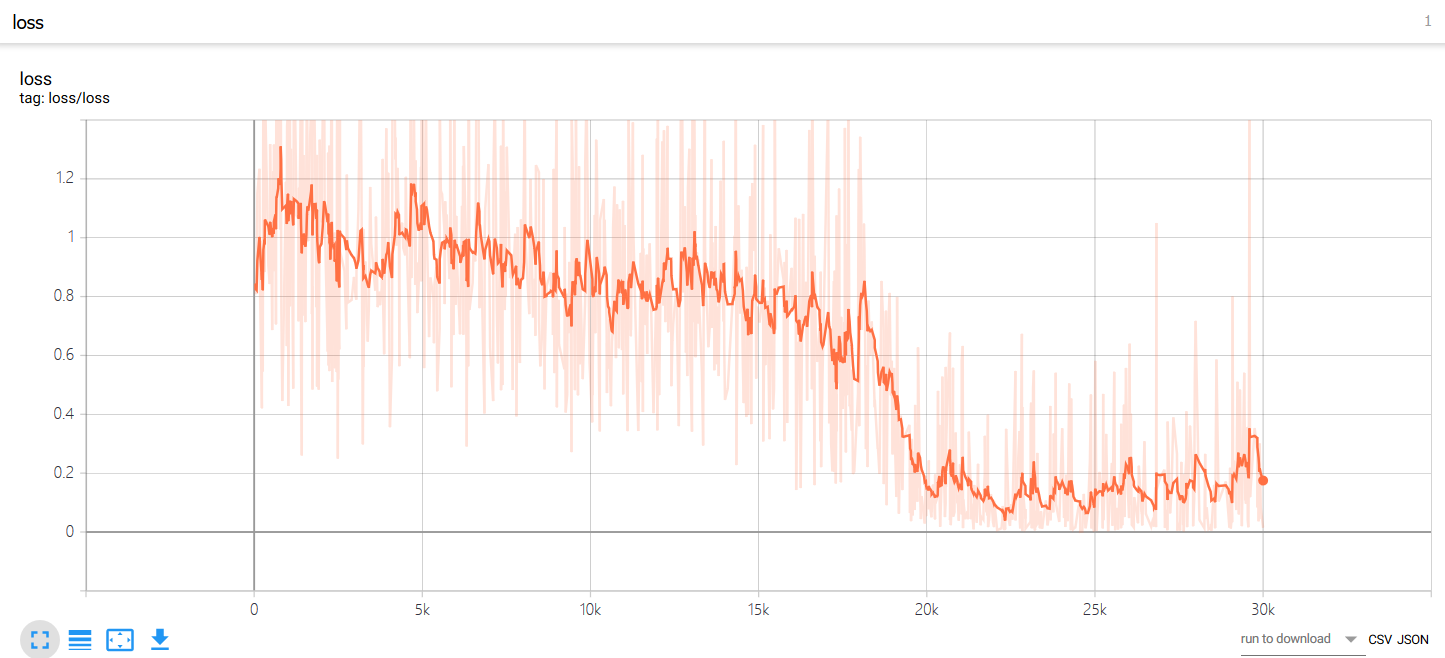
\includegraphics[width = 1\textwidth]{loss_tensorboard}
	\caption{DRQN算法Tensorboard损失曲线图}
	\label{fig:loss_tensorboard}
\end{figure}
\subsection{信道选择结果展示及分析}
首先给出使用合作式训练方法的得到的信道分配结果,如图\ref{fig:信道动作合作}所示。
\begin{figure}[htbp]
	\centering
	\includegraphics[width = 0.8\textwidth]{信道动作合作}
	\caption{DRQN合作型算法下用户选择信道结果}
	\label{fig:信道动作合作}
\end{figure}
从结果图中可以很直观的看出有两个用户长时间占用两个固定信道,有一个用户在大部分时间选择退避,不进行信息传递,显然,这样做可以使这两个信道不出现竞争冲突,频谱利用率极高。然而,根据我们日常生活经验可知,这种信道分配策略显然是不合理的,对于三个用户分配有失公允,虽然达到初始设置目标但我们认为这种方法不可取。为此我们使用上文提到的竞争型DRQN算法,每个用户都将自身累积传输奖赏最大值设为训练目标,重新进行训练,得到如图\ref{fig:信道动作竞争}所示结果。从图中可以看出在最终目标不变的情况下我们得到了一个比较有趣的结果。
\begin{figure}[htbp]
	\centering
	\includegraphics[width = 0.8\textwidth]{信道动作竞争}
	\caption{DRQN竞争型算法下用户选择信道结果}
	\label{fig:信道动作竞争}
\end{figure}
从图中可见用户1大概率占用信道1,剩余两用户竞争剩余的信道2,两者以类似于时分多址(TDMA)形式共用信道2,两者轮流进行自主退避,由此达到总传输奖赏最高,形成一种不完全的纳什均衡状态。结果可解释性较高,虽然三用户未实现完全绝对公平的信道分配,但对比合作型DRQN已经有较大程度的提升。

最后我们给出随机算法同我们使用的DRQN竞争型算法性能对比,如图\ref{fig:信道奖励对比}所示。可见DRQN算法优势明显。
\begin{figure}[htbp]
	\centering
	\includegraphics[width = 0.7\textwidth]{信道奖励对比}
	\caption{DRQN竞争型算法同随机算法性能对比结果}
	\label{fig:信道奖励对比}
\end{figure}

\section{功率控制}
\subsection{基于DRQN的智能化功率控制}
在用户结束了簇头选择以及信道选择成功建立同簇头间的通信链路之后,频谱分配任务还未结束,因为频点分配同时还应对于用户于簇头间通信功率进行控制,功率控制与信道分配相辅相成,不可分割。在进行功率控制任务时,我们仍然使用DRQN算法以及相同的网络构架。简便起见,我们只考虑两个用户在分簇模型中认知无线电框架下的次级用户功率退避问题。我们借用认知无线电中主用户和次级用户的概念进行功率问题研究,假设主用户使用固定功率调整策略如公式\ref{eq:传统功率策略}所示,出于通信安全性考虑,需要保护每个用户的通信隐私,次级用户不能直接向主用户询问通讯功率,需要通过传感器信息预测分析主用户功率,并在不影响主用户前提下选择合适的通讯功率进行通信,以减小同频干扰(当用户数量过饱和时,可能会允许多用户使用同一频道情况)或邻频干扰(用户使用邻近频道情况)。在进行仿真测验时,我们将传感器信息设置为网络输入状态,两用户物理距离采取随机产生方式生成,且只考虑自用空间损耗和高斯白噪声影响。将次级用户选取的离散功率序号作为输出动作,并对两用户使用的通信功率同初始设定SINR阈值进行对比,返回两用户传输成功数据作为奖赏反馈。仿真时超参数设置同前表\ref{tab:超参数}所示。首先我们给出DRQN网络训练的损失曲线随训练次数的变化关系,如图\ref{fig:功率loss}所示。

\begin{figure}[htbp]
	\centering
	\includegraphics[width = 0.7\textwidth]{Loss}
	\caption{DRQN算法训练损失曲线}
	\label{fig:功率loss}
\end{figure}

\begin{figure}[htbp]
	\centering
	\includegraphics[width = 0.7\textwidth]{Success}
	\caption{DRQN算法测试成功率曲线}
	\label{fig:功率success}
\end{figure}
\subsection{功率控制结果展示及分析}
为了展示训练后智能体功率控制效果,我们引入两个比较参数,首先是$Success=\frac{success\_number}{test\_number}$用来表示使用算法可以最终达到理想共存状态$SINR_{i}\geqslant\eta_{i}$的成功比例,结果如图\ref{fig:功率success}所示。

可见随训练进行成功率整体上升,但稍有些不稳定。第二个参数$Used\_step$表示每次尝试从初始状态达到理想共存状态时需要使用的平均交互次数,结果如图\ref{fig:功率step}所示,可见随训练进行,智能体达到理想共存状态所需的时间逐步减少,表明智能体效率逐步增加。
\begin{figure}[htbp]
	\centering
	\includegraphics[width = 0.7\textwidth]{step number}
	\caption{DRQN算法测试平均耗时曲线}
	\label{fig:功率step}
\end{figure}

\section{基于DRQN的异构系统频谱分配存在的问题及后续工作方向}
通过上面的结果展示我们可以看出,DRQN这种深度强化学习在应对频谱分配问题上拥有不错的效果,但通过认真的分析和反思,我就发现的一些问题和不足进行阐述,并给出后续工作的方向展望。首先,对于异构系统分簇构架下的频谱分配问题,虽然我们在地面段创新性的提出了以用户为中心的分簇模型,很好的解决了地面段频谱资源的分配,但对于卫星和空中无人机平台的研究还需要进一步跟进,比如卫星间协同工作问题以及无人机资源卸载问题,同时在物理层面高频段电波信号的损耗问题以及网络层不同系统协议同一问题等需要进一步研究完善。另外对于异构用户的评价体系也为给出详细具体的实施方案,仅仅使用QoS是远远不够的,近年来有学者研究的使用QoE作为评价指标可能是解决方案。至于资源分配算法层面,我们使用的DRQN算法虽然让DQN网络具有时序预测能力,但DQN方法本身固有缺陷并未克服,比如训练难度大,易陷入局部最优解。

对于我们的项目,这里也有需要后续改进地方,比如虽然在解决簇头选择,信道分配,功率控制时使用的都是同一算法与同一网络框架,但由于三个问题具体细节的不同使得三个网络不能共享网络参数,实现同步训练,后续将其统一与结合将是待解决问题。另外目前算法仍存在性能上提高的空间,比如在解决簇头选择问题时,当簇头状态变化剧烈程度超过网络预测能力时,DRQN算法预测效果将会大打折扣;在解决信道分配时,随用户数量增加网络变得更难收敛;解决功率控制问题时,智能体稳定性稍弱。这些问题的存在使得整个网络框架运作起来效果不尽如人意,仍需后续 工作进行补充和完善。

\section{本章小结}
本章对DRQN算法具体应用进行了详细论述,对异构系统频谱分配问题从仿真层面进行了具体阐述,对簇头选择,信道选择,功率控制三个问题进行了算法应用和仿真,并对结果分别进行展示和分析。在最后对整体项目存在的问题以及对于未来工作方向进行了展望,提出了自己的意见。





















%\chapter{图片}
%
%
%\section{引言}
%
%\section{普通图片}
%
%\subsection{示例}
%
%\subsection{深度强化学习}
%\begin{figure}[h]
%	\centering
%	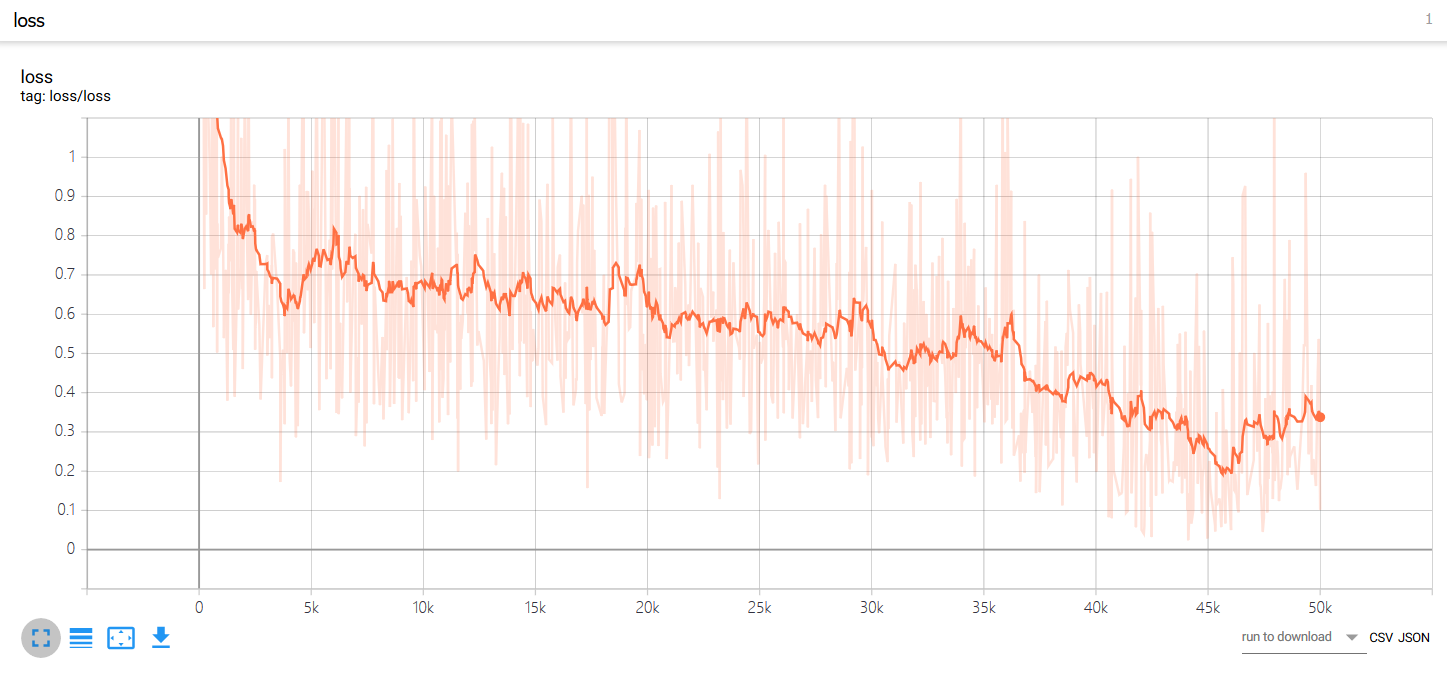
\includegraphics[width = 0.8\textwidth]{频道选择,损失,tensorboard}
%	\caption{频道选择,损失,tensorboard}
%	\label{fig:channel choose loss tensorboard}
%\end{figure}
%
%\subsection{深度强化学习}
%\begin{figure}[h]
%	\centering
%	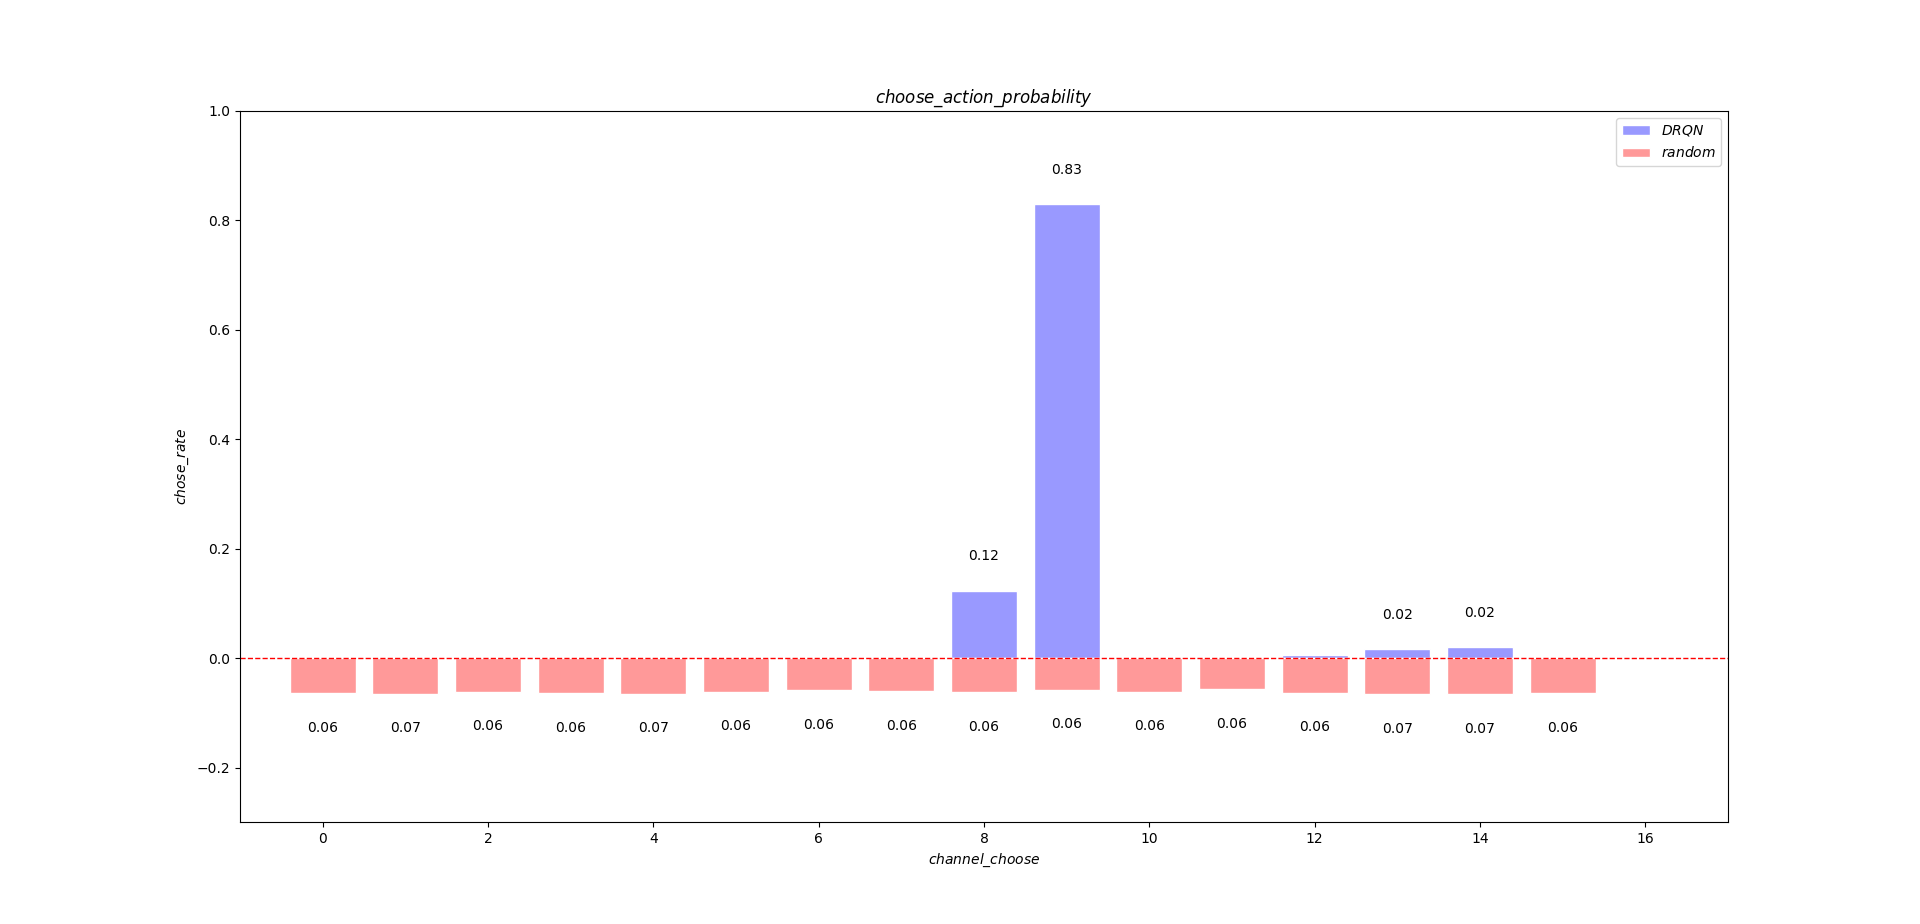
\includegraphics[width = 0.8\textwidth]{动作概率,条形图}
%	\caption{动作概率,条形图}
%\end{figure}
%
%这里引用了一个图片\ref{fig:vaeinput}.
%这里再次引用了一个图片\ref{fig:channel choose loss tensorboard}.
%
%\begin{figure}[htbp]
%	\begin{minipage}{\textwidth}
%		\centering
%		\subfigure{\label{fig:vaeinput}}\addtocounter{subfigure}{-2}
%		\subfigure{\subfigure[输入的图片]{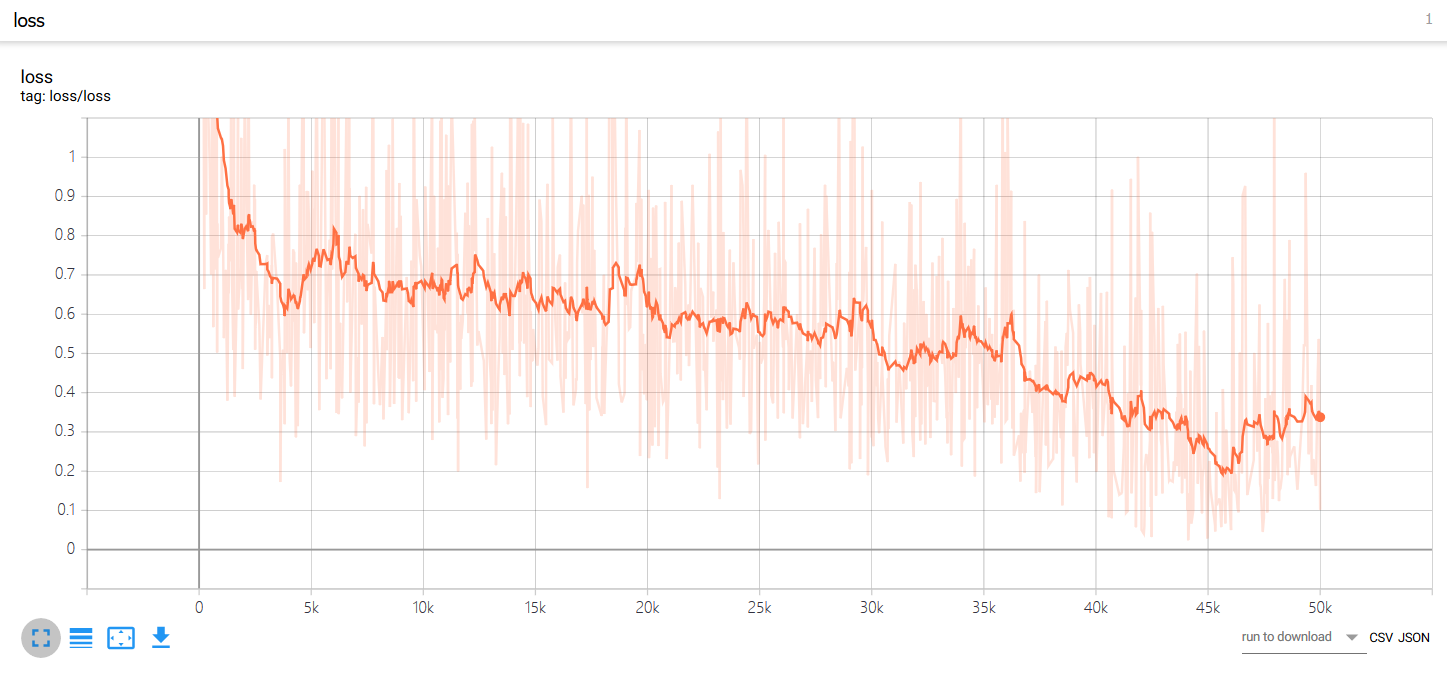
\includegraphics[width=0.2\textheight]{频道选择,损失,tensorboard}}}
%		\hspace{1em}
%		\subfigure{\label{fig:vaeinput2}}\addtocounter{subfigure}{-2}
%		\subfigure{\subfigure[输入的图片2]{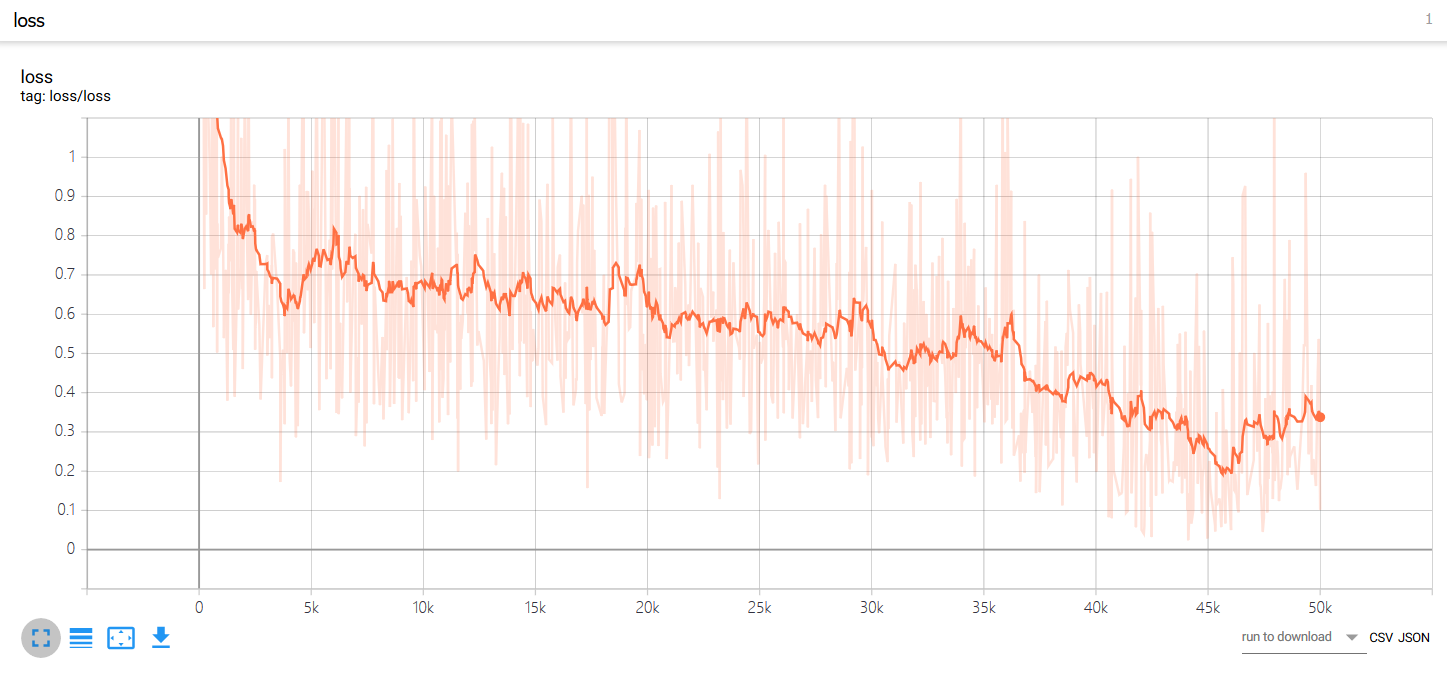
\includegraphics[width=0.2\textheight]{频道选择,损失,tensorboard}}}
%		\hspace{1em}
%		\subfigure{\label{fig:vaeinput3}}\addtocounter{subfigure}{-2}
%		\subfigure{\subfigure[输入的图片3]{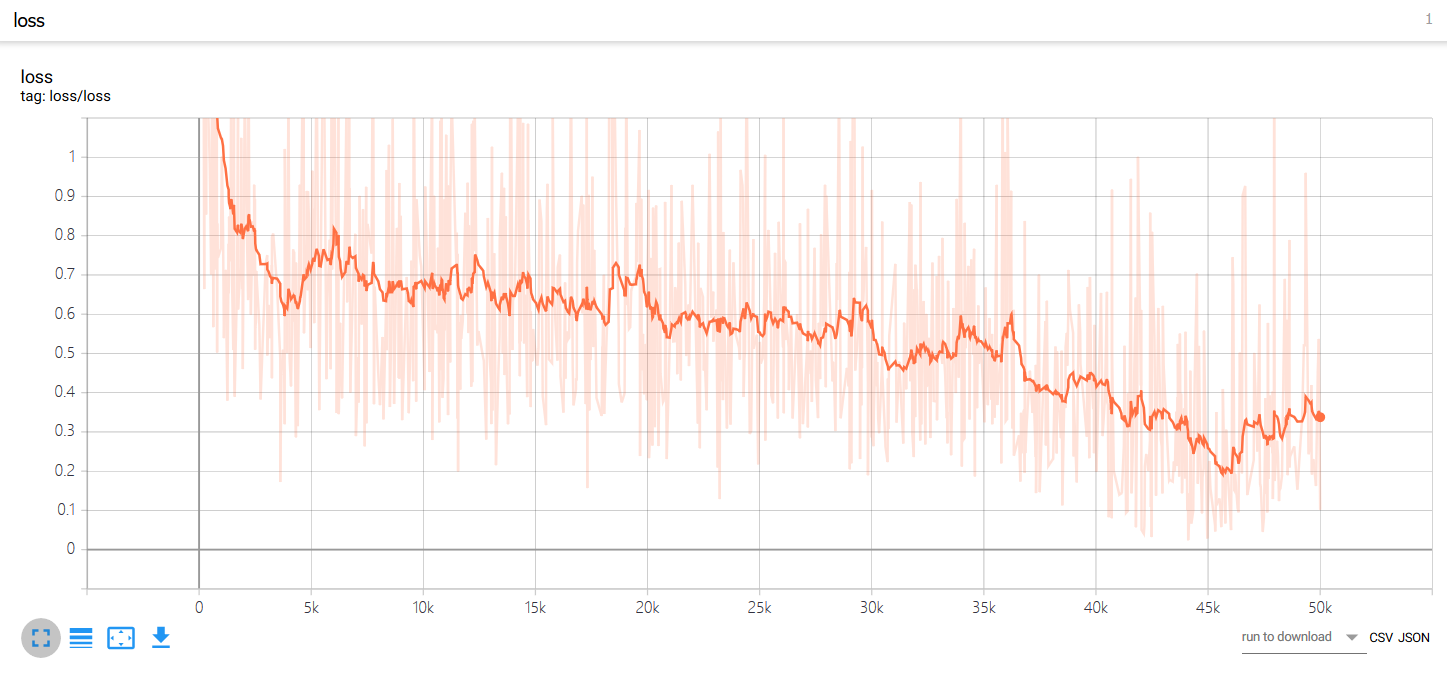
\includegraphics[width=0.2\textheight]{频道选择,损失,tensorboard}}}
%		\hspace{1em}
%		\subfigure{\label{fig:vaeinput4}}\addtocounter{subfigure}{-2}
%		\subfigure{\subfigure[输入的图片4]{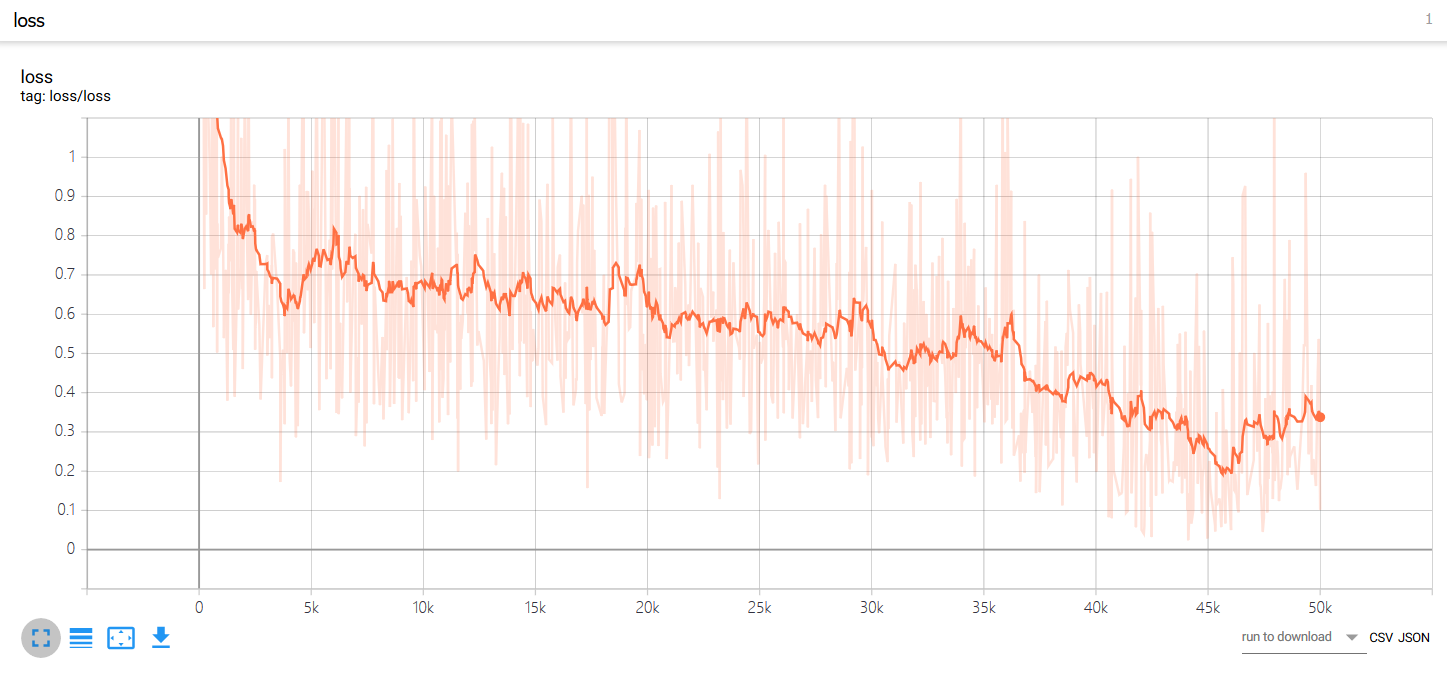
\includegraphics[width=0.2\textheight]{频道选择,损失,tensorboard}}}
%	\end{minipage}
%	\vspace{0.2em}
%\caption{输入图片对比}\label{fig:vaemnist}
%\end{figure}
%
%
%
%\chapter{表格}
%
%\begin{table}[htbp]
%	\caption{一个表格}\label{tab:一个表格}
%	\vspace{0.5em}\centering\wuhao
%	\begin{tabular}{ccccc}
%		\toprule[1.5pt]
%		$D$(in) & $P_u$(lbs) & $u_u$(in) & $\beta$ & $G_f$(psi.in)\\
%		\midrule[1pt]
%		5 & 269.8 & 0.000674 & 1.79 & 0.04089\\
%		10 & 421.0 & 0.001035 & 3.59 & 0.04089\\
%		20 & 640.2 & 0.001565 & 7.18 & 0.04089\\
%		\bottomrule[1.5pt]
%	\end{tabular}
%\end{table}
%
%
%
%\section{本章小结}